\section{Grundkonzept}
\begin{figure}[h]
	\centering
	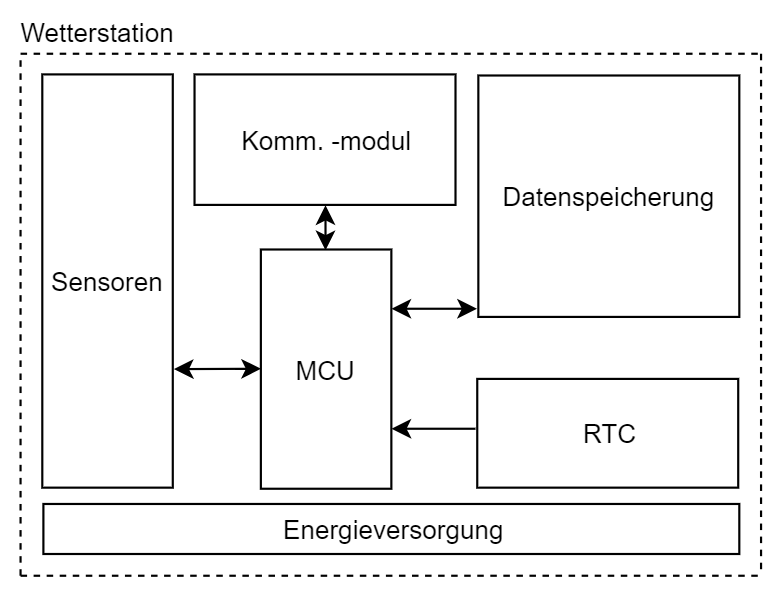
\includegraphics[width=0.9\textwidth]{graphics/Grundkonzept.PNG}
	\caption{Grundkonzept}
	\label{fig:grundkonzept}
\end{figure}

\paragraph{Übersicht:}
Als Zentralrecheneinheit wird eine \textit{Micro-Controller-Unit (MCU)} verwendet. Dieser ist dafür verantwortlich, dass die Daten richtig verarbeitet und an das dementsprechende Modul weitergeleitet werden. Die Messdaten werden in digitaler Form vom Modul \textit{Sensoren} an die \textit{MCU} übertragen. Dieser fügt mit dem \textit{Real-Time-Clock (RTC)} einen Timestamp hinzu, wobei anschließend die Daten in der \textit{Datenspeicherung} nichtflüchtig gespeichert werden. Über das \textit{Kommunikationsmodul} können dann die Daten von Nutznießern abgefragt werden.

\vspace{0.5cm}
\hrule
\vspace{0.25cm}

Das gesamte Grundkonzept ist, wie in der Abbildung \ref{fig:grundkonzept} graphisch Dargestellt, modular aufgebaut. Auf alle einzelnen Module wird folgend spezifischer eingegangen und die Konzeptvariationen vorgestellt.
\newpage
\subsection{Micro Controller Unit (MCU)}

\newpage
\subsection{Sensoren}
\begin{figure}[h]
\centering
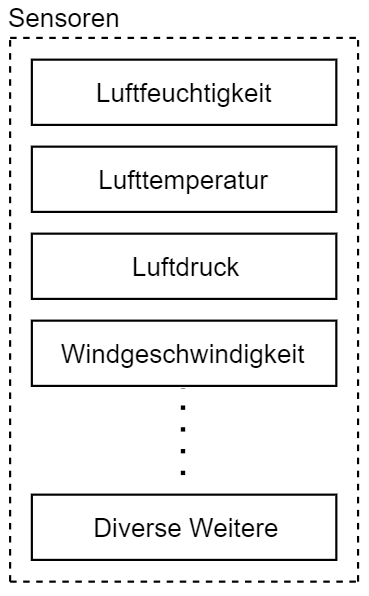
\includegraphics[scale=0.8]{graphics/Sensoren.PNG}
\caption{Sensoren}
\end{figure}

\subsubsection*{Sensoraufbau}
\begin{figure}[h]
\centering
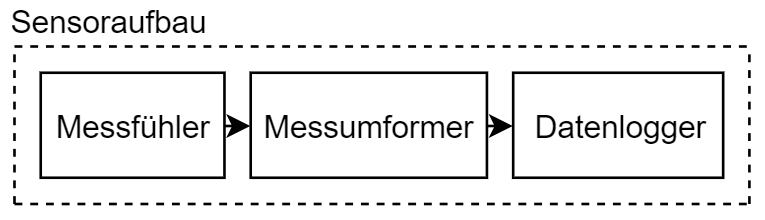
\includegraphics[scale=0.7]{graphics/Sensoraufbau.PNG}
\caption{Sensoraufbau}
\end{figure}

\subsubsection{Temperatursensor}


\subsubsection{Luftfeuchtigkeitssensor}
Die Bestimmung der relativen Luftfeuchtigkeit spielt eine markante Rolle in der Meteorologie. Dieser Wert sagt aus, wie sehr die Luft mit Wasserdampf gesättigt ist und wird mit anderen Faktoren benutzt um zuverlässige lokale Wetterprognosen zu erstellen. Die Normwerte für die Schweiz liegen ungefähr zwischen 58 und 92 Prozent relativer Luftfeuchtigkeit  \cite{MeteoSchweizFeuchte}.\\
Um diesen Wert zu messen, wird ein kapazitiver Absorptionshygrometer verwendet. Diese sind weit verbreitet, besitzen eine passable Genauigkeit (1-3 \% relative Luftfeuchte), sind Robust, wartungsarm und kostengünstig.

\subsubsection{Luftdrucksensor}
Der Luftdruck spielt bei der Erkennung von Hoch- und Tiefdruckgebieten eine wichtige Rolle in der Meteorologie. Diser wird ebenso verwendet um zuverlässige lokale Wetterprognosen zu erstellen. Die Normwerte für die Schweiz liegen ungefähr zwischen 640 und 1000 hPa \cite{MeteoSchweizDruck}.\\
Um diesen Wert zu messen, wird ein Absolutdrucksensor benötigt, welcher den Absolutwert des aufgenommenen Drucks durch Vergleich mit Vakuum als Referenzpunkt ermittelt. Dieses Verfahren ist die einzige Möglichkeit um den atmosphärischen Luftdruck selbst zu messen \cite{WikiDruck}. 

\subsubsection{Windstärke- und Windrichtungssensor}
Die Windstärke (Windgeschwindigkeit) und Windrichtung haben einen Einfluss auf das Wetter und sind aus diesem Grund ebenso von Bedeutung für die Meteorologie. Ausserdem indizieren hohe Windstärke Stürme, weshalb vor allem die Windstärkemessung für Unwetterwarnungen von hoher Bedeutung ist. Die Normwerte für die Schweiz liegen ungefähr zwischen 0.5 und 11 $\frac{m}{s}$ \cite{MeteoSchweizWindnorm}. Wobei bereits Extremwerte mit bis zu 53 $\frac{m}{s}$ im Flachland und bis zu 75 $\frac{m}{s}$ in den Bergen detektiert wurden \cite{MeteoSchweizExtrem}.\\
Um die Windstärke zu messen, wird ein Schalenanemometer verwendet, da diese nicht nach der Windrichtung ausgerichtet werden müssen und nicht so viel Strom benötigen wie auf Ultraschall basierende Sensoren. Die Windrichtung selbst kann mit einer Windfahne detektiert werden, wobei hier die Umsetzung der Richtung in ein digitales Signal weitere Recherche benötigt.

\subsubsection{Niederschlagsensor}


\newpage
\subsection{Kommunikationsmodul}
\begin{figure}[h]
\centering
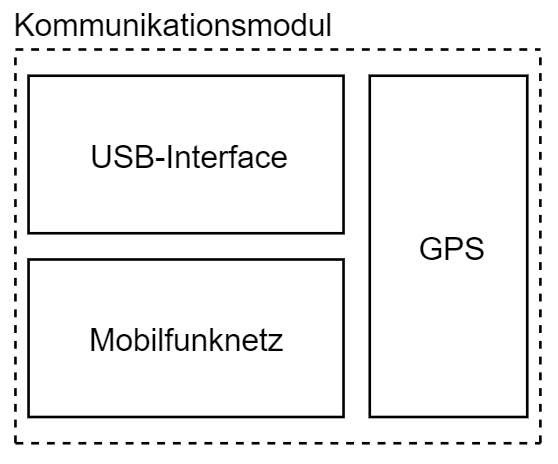
\includegraphics[scale=0.7]{graphics/Kommunikationsmodul.PNG}
\caption{Kommunikationsmodul}
\end{figure}

\newpage
\subsection{Datenspeicherung}

\newpage
\subsection{RTC}

\newpage
\subsection{Speisung}
\begin{figure}[h]
\centering
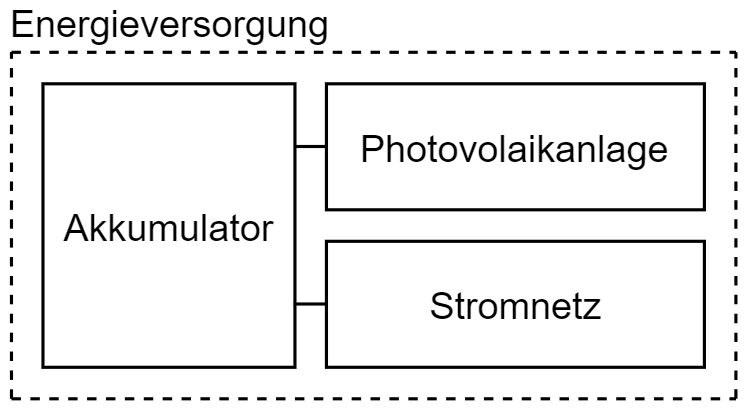
\includegraphics[scale=0.6]{graphics/Energieversorgung.PNG}
\caption{Energieversorgung}
\end{figure}
